\documentclass[border=10pt, tikz]{standalone}
\usetikzlibrary{arrows.meta, positioning, calc}

% Define colors from the user-provided Leibniz rule
\definecolor{interiorCol}{HTML}{00d1b2} % Teal
\definecolor{fminusCol}{HTML}{4facfe}   % Sky Blue (Upper bound logic)
\definecolor{fplusCol}{HTML}{ff6b6b}    % Coral Red (Lower bound logic)
\definecolor{textdark}{HTML}{222222}
\definecolor{curveblue}{HTML}{9CCBE3}

\begin{document}
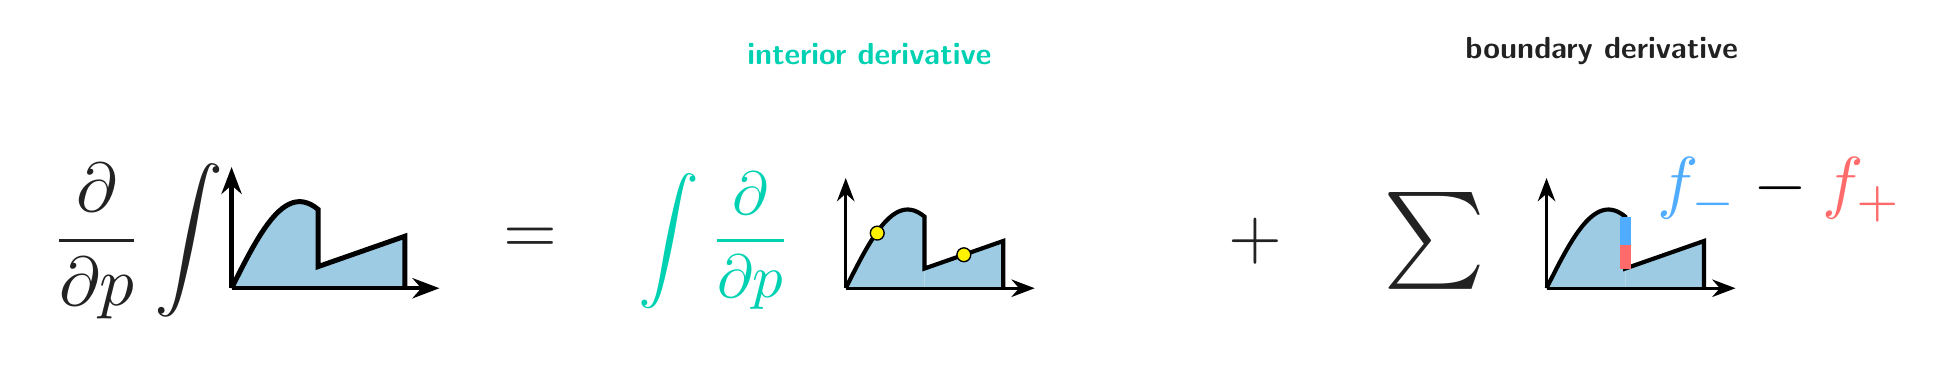
\begin{tikzpicture}[
    font=\sffamily,
    >=Stealth,
    mathnode/.style={scale=2.5, text=textdark, anchor=center},
    labelnode/.style={scale=1.1, font=\sffamily\bfseries, anchor=south}
]

% --- 1. LEFT HAND SIDE (LHS) ---
\node[mathnode] (LHS_SYM) at (0, 1.1) {$\displaystyle \frac{\partial}{\partial p} \int$};

\begin{scope}[shift={(1.2, 0.5)}, scale=0.55]
    \fill[curveblue] (0,0) -- plot[domain=0:2] (\x, {2*sin(\x r)}) -- (2,0) -- cycle;
    \fill[curveblue] (2,0) -- (2, 0.5) -- (4, 1.2) -- (4, 0) -- cycle;
    \draw[line width=1.5pt, ->] (0,0) -- (4.8,0);
    \draw[line width=1.5pt, ->] (0,0) -- (0,2.8);
    \draw[line width=1.8pt] (0,0) -- plot[domain=0:2] (\x, {2*sin(\x r)}) -- (2,0.5) -- (4, 1.2) -- (4, 0);
\end{scope}

% --- 2. EQUALS SIGN ---
\node[mathnode] at (5.0, 1.1) {$=$};

% --- 3. INTERIOR DERIVATIVE SECTION ---
\begin{scope}[shift={(5.8, 0)}]
    \node[labelnode, interiorCol] at (3.5, 3.2) {interior derivative};
    
    \node[scale=2.2, anchor=west, interiorCol] at (0.3, 1.1) {$\displaystyle \int \frac{\partial}{\partial p}$};
    
    \begin{scope}[shift={(3.2, 0.5)}, scale=0.5]
        \fill[curveblue] (0,0) -- plot[domain=0:2] (\x, {2*sin(\x r)}) -- (2,0) -- cycle;
        \fill[curveblue] (2,0) -- (2, 0.5) -- (4, 1.2) -- (4, 0) -- cycle;
        \draw[line width=1.2pt, ->] (0,0) -- (4.8,0);
        \draw[line width=1.2pt, ->] (0,0) -- (0,2.8);
        \draw[line width=1.5pt] (0,0) -- plot[domain=0:2] (\x, {2*sin(\x r)}) -- (2,0.5) -- (4, 1.2) -- (4, 0);
        \fill[yellow, draw=black, line width=0.5pt] (0.8, 1.4) circle (5pt);
        \fill[yellow, draw=black, line width=0.5pt] (3.0, 0.85) circle (5pt);
    \end{scope}
\end{scope}

% --- 4. PLUS SIGN ---
\node[mathnode] at (14.2, 1.1) {$+$};

% --- 5. BOUNDARY DERIVATIVE SECTION ---
\begin{scope}[shift={(15.1, 0)}]
    \node[labelnode, textdark] at (3.5, 3.2) {boundary derivative};
    
    \node[scale=3.5, anchor=west, textdark] at (0.3, 1.1) {$\sum$};
    
    \begin{scope}[shift={(2.8, 0.5)}, scale=0.5]
        \fill[curveblue] (0,0) -- plot[domain=0:2] (\x, {2*sin(\x r)}) -- (2,0) -- cycle;
        \fill[curveblue] (2,0) -- (2, 0.5) -- (4, 1.2) -- (4, 0) -- cycle;
        \draw[line width=1.2pt, ->] (0,0) -- (4.8,0);
        \draw[line width=1.2pt, ->] (0,0) -- (0,2.8);
        \draw[line width=1.5pt] (0,0) -- plot[domain=0:2] (\x, {2*sin(\x r)}) -- (2,0.5) -- (4, 1.2) -- (4, 0);
        
        % Boundary Jump Visualization
        \draw[fminusCol, line width=4pt] (2, 1.1) -- (2, 1.8);
        \draw[fplusCol, line width=4pt] (2, 0.5) -- (2, 1.1);
        
        % Math Notation with specific colors
        \node[anchor=west, scale=2.5] at (2.2, 2.5) {${\color{fminusCol}f_-} - {\color{fplusCol}f_+}$};
    \end{scope}
\end{scope}

\end{tikzpicture}
\end{document}